\documentclass[linenumbers]{aastex631}
\usepackage{amsmath,tikz}
\usetikzlibrary{matrix}
\newcommand{\vdag}{(v)^\dagger}
\newcommand\aastex{AAS\TeX}
\newcommand\latex{La\TeX}
\begin{document}

\title{Demonstração Schrodinger-Crank-Nicolson}

\author[0000-0002-2462-9263]{Gabriel Siqueira}
\affiliation{Centro Federal de Educação Tecnológica de Minas Gerais}

\section{Introdução} \label{sec:intro}

Utilizado para simplificar equações diferenciais parciais, nesse caso a equação de Schrodinger:

\begin{equation}
    i\cdot\hbar\frac{\partial\psi(x,t)}{\partial t}=-\frac{\hbar^2}{2m}\frac{\partial^2\psi(x,t)}{\partial x^2} + V(x,t)\psi(x,t)
\end{equation}

Na análise numérica, o método de Crank-Nicolson mostra que a derivada parcial pode ser aproximada por uma secante, portanto é possível estabelecer uma diferença conforme visto na definição de derivada sem a utilidade do limite (dessa forma a variação do denominador não será nula o suficiente para termos uma tangente).

\begin{equation}
    \frac{\psi^{n+1}_i-\psi^{n}_i}{\Delta t}
\end{equation}

Mas como alcançar a equação (2)?

\section{O método das diferenças finitas}

Utilizado para resolver problemas com valor inicial ou problemas de contorno para EDO e EDP, usaremos para lidar com a EDP da equação 1. Como são EDP's podemos dizer que a nossa variável independente da equação é x e a tarefa é discretizá-la (Dividir em subdomínios). Para um domínio semi-infinito os subdomínios podem ser representados como, 0, 1, 2, ..., i - 1, i, i + 1.

O próximo passo é gerar as aproximações para obter $\dot\psi_i$ e $\ddot\psi_i$ nos pontos discretos $x_i$ utilizando $\psi$. Após a aproximação, aplica-se a EDP gerando sistemas de equações álgebra na forma: f($\psi_i$)=0, tal f é o vetor das equações álgebricas que depende de valores de $\psi_i$. De fato, a aplicação do método da discretizaçção se resolve localmente, em cada $x_i$ e o seu resultado é um conjunto enumerável.

\section{Aproximação de derivadas}

Como as diferenças finitas são usadas para resolver equações diferenciais, podemos expandir em série de Taylor em torno de um dado ponto. Então seja $\psi(x_{i+1}) = \psi_{i+1}$, então o valor de $\psi_{i+1}$ pode ser definido como:

\begin{equation}
    \psi_{i+1} = \psi_i+\dot\psi_i(x_{i+1}-x_{i})+\ddot\psi_i\frac{(x_{i+1}-x_i)^2}{2}+...
\end{equation}

Enquanto que, para $\psi(x_{i-1})=\psi_{i-1}$

\begin{equation}
    \psi_{i-1} = \psi_i-\dot\psi_i(x_{i}-x_{i-1})+\ddot\psi_i\frac{(x_{i-1}-x_i)^2}{2}+...
\end{equation}

\section{Comprimento do domínio}

\begin{equation}
    h_i=x_i-x_{i-1}
\end{equation}

A equação se torna mais comapcta e melhor para demonstrar. Com o objetivo de isolar a primeira derivada e limitar as superiores podemos:

\begin{equation}
    h^2_i\psi_{i+1}-h^2_{i+1}\psi_{i-1} = (h^2_i-h^2_{i+1})\psi_i+(h^2_ih_{i+1}+h_ih^2_{i+1})\dot\psi_i+\ddot\psi_i(h^2_ih^2_{i+1}-h^2_{i+1}h^2_i)+...
\end{equation}

Com essa subtração, o termo de segundo grau sumirá, e isso é importante, visto que há um solução para ele. Isolando a primeira derivada obtemos:

\begin{equation}
    \dot\psi_i = \frac{h^2_i\psi_{i+1}+(h^2_{i+1}-h^2_i)\psi_i-h^2_{i+1}\psi_{i-1}}{h^2_ih_{i+1}+h_ih^2_{i+1}} + O\left(\frac{\texttt{Taylor's series \geq 3}}{h^2_ih_{i+1}+h_ih^2_{i+1}}\right)
\end{equation}

E O indica as outras séries que quando seu valor tende a 0 significa que teremos uma derivada exata. Chamamos isso de erro de truncamento. Para a nossa aproximação ignoraremos o erro de truncamento.

\section{Malha uniforme}

Em uma malha uniforme a diferença no domínio em i, dada por h é a mesma, ou seja:

\begin{equation}
    h_i=h, \forall i
\end{equation}

Portanto:

$$\dot\psi_i = \frac{h^2\psi_{i+1}+(h^2-h^2)\psi_i-h^2\psi_{i-1}}{h^2h+hh^2} = \frac{\psi_{i+1}-\psi_{i-1}}{2h}$$

E essa é a diferença central da primeira derivada. Como é uma malha uniforme, a diferença é a mesma:

\begin{equation}
    \frac{\psi_{i+1}-\psi_i}{h} = \frac{\psi_i-\psi_{i-1}}{h}
\end{equation}

O próximo passo é obter para a segunda derivada sumindo com a primeira derivada. Assim $h_i$ multiplica $\psi_{i+1}$, $h_{i+1}$, $\psi_{i-1}$.

\begin{equation}
    h_i\psi_{i+1}-h_{i+1}\psi_{i-1} = (h_i-h_{i+1})\psi_i+(h_ih_{i+1}+h_ih_{i+1})\dot\psi_i+\ddot\psi_i(h_ih^2_{i+1}+h_{i+1}h^2_i)+...
\end{equation}

Isolando o $\ddot\psi_i$:

\begin{equation}
    \ddot\psi_i = \frac{h_i\psi_{i+1}-(h_{i+1}+h_i)\psi_i+h_{i+1}\psi_{i-1}}{\frac{h^2_{i+1}h_i+h_{i+1}h^2_i}{2}} + O\left(\frac{\texttt{Taylor's series \geq 3}}{\frac{h^2_{i+1}h_i+h_{i+1}h^2_i}{2}}\right)
\end{equation}

Portanto, tendendo $z \rightarrow 0$ e $h_i=h$, obtemos:

\begin{equation}
    \ddot\psi_i=\frac{\psi_{i+1}-2\psi_i+\psi_{i-1}}{h^2}
\end{equation}

\section{Além do implícito e explícito}

Crank-Nicolson é justamente um método para segundo grau no tempo e espaço. Provadamente estável então é uma ótima aproximação para a tarefa.

$$f_{i+1/2}=\frac{1}{2}(f_i+f_{i+1})$$
$$f_{i+1/2}=1/2(f(t_i,y_i)+f(t_{i+1},y_{i+1}))$$

Em (11) obtemos o caso para a segunda derivada então basta substituir, supondo que f seja a segunda derivada de uma função. Então para Crank-Nicolson a segunda derivada equivale à:

\begin{equation}
    \frac{1}{2}\cdot\frac{y^t_{i+1}-2y^t_i+y^t_{i-1}+y^{t+1}_{i+1}-2y^{t+1}_i+y^{t+1}_{i-1}}{h^2}
\end{equation}

Então a variação no tempo existe para um espaço homogêneo.

\section{Representação algébrica}

Dada a equação 1 deste trabalho, podemos reintrepretá-la como:

\begin{equation}
    \frac{\partial\psi(x,t)}{\partial t} = \frac{\psi^{n+1}_i - \psi^n_i}{\Delta t}
\end{equation}

\begin{equation}
    \frac{\partial^2\psi(x,t)}{\partial x^2} = \frac{1}{2\Delta x^2}[(\psi^{n+1}_{i+1} - 2\psi^{n+1}_{i}+\psi^{n+1}_{i-1})+(\psi^{n}_{i+1} - 2\psi^{n}_{i}+\psi^{n}_{i-1})]
\end{equation}

\begin{equation}
    V(x,t)\psi(x,t)=1/2[V^{n+1}_i\psi^{n+1}_i+V^{n}_i\psi^{n}_i]
\end{equation}

\begin{equation}
    \frac{i\hbar}{\Delta t}[\psi^{n+1}_i - \psi^n_i]=\frac{-\hbar^2}{4m\Delta x^2}[(\psi^{n+1}_{i+1} - 2\psi^{n+1}_{i}+\psi^{n+1}_{i-1})+(\psi^{n}_{i+1} - 2\psi^{n}_{i}+\psi^{n}_{i-1})]+\frac{1}{2}[V^{n+1}_i\psi^{n+1}_i+V^{n}_i\psi^{n}_i]
\end{equation}

Para fins de simplificação utilizaremos $a = \frac{-\hbar^2}{4m\Delta x^2}$, dessa forma:

$$\frac{i\hbar}{\Delta t}\psi^{n+1}_i-2a\psi^{n+1}_i-\frac{1}{2}V^{n+1}_i\psi^{n+1}_i = \frac{i\hbar}{\Delta t}\psi^{n}_i-2a\psi^{n}_i-\frac{1}{2}V^{n}_i\psi^{n}_i-a\psi^{n+1}_{i+1}-a\psi^{n+1}_{i-1}-a\psi^{n}_{i+1}-a\psi^{n}_{i-1}$$

E para melhorar a solução podemos observar a evidência de $\psi^{n}_i$ e $\psi^{n+1}_i$ e destacar que:

\begin{equation}
    b_i=\frac{i\hbar}{\Delta t} - 2a - 1/2V^{n+1}_i
\end{equation}
\begin{equation}
    c_i=\frac{i\hbar}{\Delta t} + 2a + 1/2V^{n}_i
\end{equation}
\begin{equation}
    a\psi^{n+1}_{i+1}+b_i\psi^{n+1}_i+a\psi^{n+1}_{i-1}=-a\psi^{n}_{i+1}+c_i\psi^{n+1}_i-a\psi^{n}_{i-1} 
\end{equation}

Assim obtemos quatro matrizes capazes de estabelecer uma relação, mesmo que incompleta, $A\psi^{k+1}_i = B\psi^{k}_i$, onde:

\begin{equation}
    A\psi^{k+1}=
    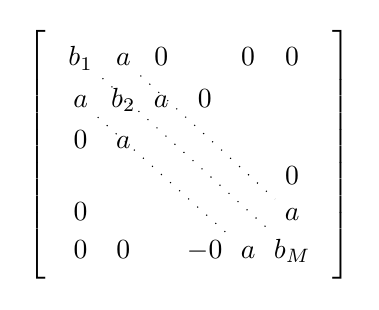
\begin{tikzpicture}[baseline=(current bounding box.center)]
    \matrix (m) [matrix of math nodes,nodes in empty cells,right delimiter={]},left delimiter={[} ]{
    b_1  & a & 0  &  & 0 & 0  \\
    a  & b_2 & a & 0 \\
    0 & a & & &    \\
       & & & & & 0  \\
    0  & & & & & a \\
    0 &0 & & -0 & a & b_M\\
    } ;
    \draw[loosely dotted] (m-1-1)-- (m-6-6);
    \draw[loosely dotted] (m-1-2)-- (m-5-6);
    \draw[loosely dotted] (m-2-1)-- (m-6-5);
    \end{tikzpicture}
    \begin{pmatrix}
        \psi^{k+1}_0\\\psi^{k+1}_1\\\vdots\\\psi^{k+1}_M
    \end{pmatrix}
\end{equation}

\begin{equation}
    B\psi^{k}=
    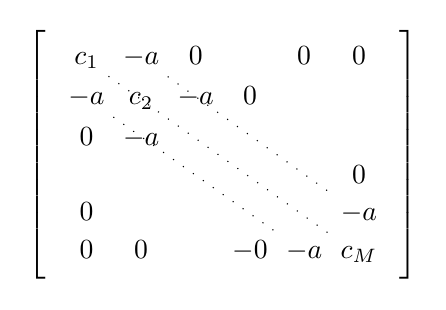
\begin{tikzpicture}[baseline=(current bounding box.center)]
    \matrix (m) [matrix of math nodes,nodes in empty cells,right delimiter={]},left delimiter={[} ]{
    c_1  & -a & 0  &  & 0 & 0  \\
    -a  & c_2 & -a & 0 \\
    0 & -a & & &    \\
       & & & & & 0  \\
    0  & & & & & -a \\
    0 &0 & & -0 & -a & c_M\\
    } ;
    \draw[loosely dotted] (m-1-1)-- (m-6-6);
    \draw[loosely dotted] (m-1-2)-- (m-5-6);
    \draw[loosely dotted] (m-2-1)-- (m-6-5);
    \end{tikzpicture}
    \begin{pmatrix}
        \psi^{k}_0\\\psi^{k}_1\\\vdots\\\psi^{k}_M
    \end{pmatrix}
\end{equation}

\end{document}
